%!TEX root = Zwischen-ML-Prak-2015.tex
\section{Lessons learned}

\subsection{Caffe}

\begin{frame}{Erste Ergebnisse}

\centering

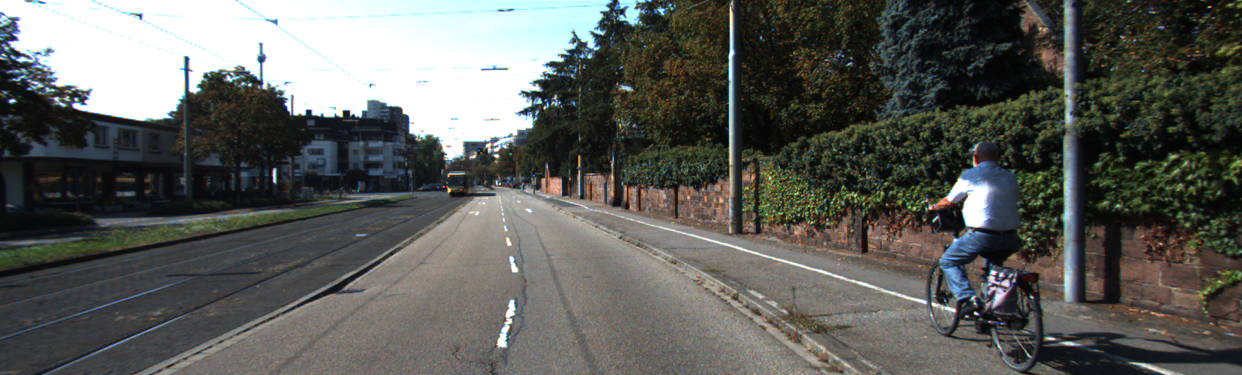
\includegraphics[width=0.75\textwidth]{../images/um_000000.png}

\hspace{0.5cm}

\only<1>{
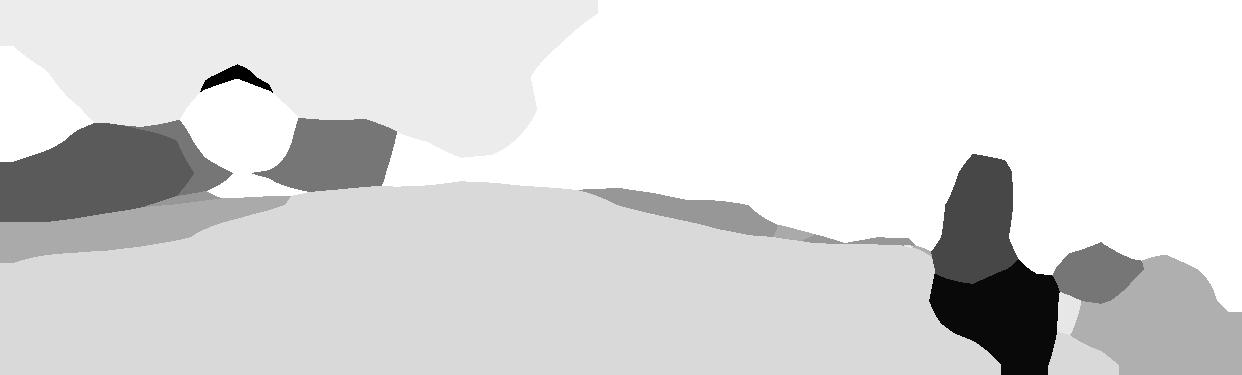
\includegraphics[width=0.75\textwidth]{../images/um-segmentation.png}
}

\only<2>{
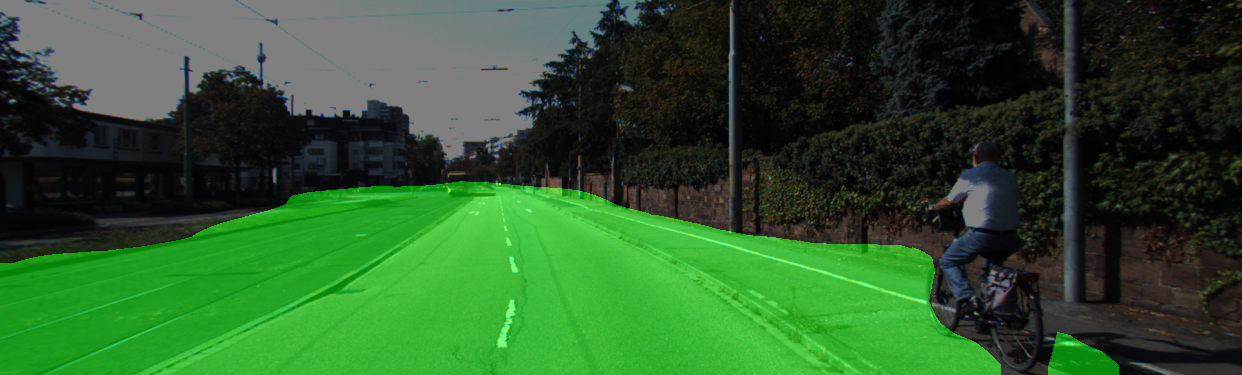
\includegraphics[width=0.75\textwidth]{../images/um-overlay.png}
}

 %TODO: Komische Fehler (TODO: ein paar einbinden)

\end{frame}

\begin{frame}{Challenges}

\centering

\begin{itemize}
 \item Reduziere Netzgröße (von 11.5 GiB) \\
 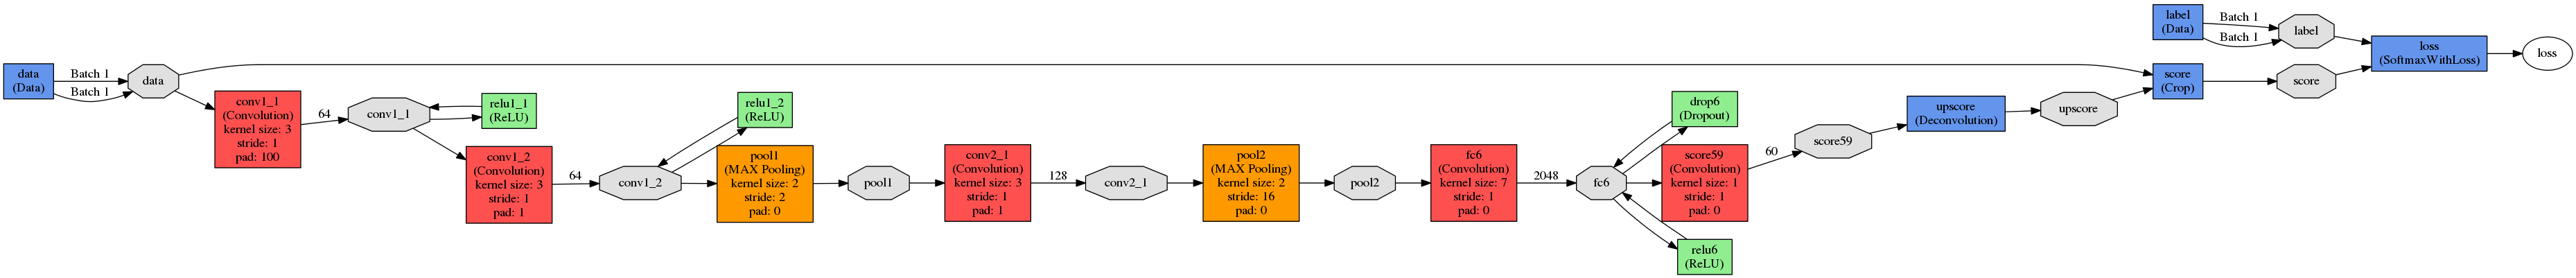
\includegraphics[width=0.9\textwidth]{../images/mid.png}
 \item trainiere mit Eigenen Daten \\
 \begin{minipage}{0.45\textwidth}
 
\includegraphics[width=\textwidth]{../images/out.png}
 \end{minipage}  \begin{minipage}{0.45\textwidth}
 
\includegraphics[width=\textwidth]{../images/out-um.png}  
 \end{minipage}
\end{itemize}
\end{frame}